\section{Introduction}
\label{sec:intro}

% P1: need and the dominant design (A/B round 1: judged clearly better than the LongMemEval opening; edits applied)
A chat assistant that has talked with a user for months accumulates more history than the answering model can
read in a single context. In the 1M-token tier of BEAM~\citep{tavakoli2025beam}, one conversation spans about
1,700 turns and 530,000 words. Its questions ask for the user's current plan, whether two of their statements
contradict each other, or how a project evolved over several months. Memory systems address such questions by
storing a compact version of the history and retrieving from it when a question
arrives~\citep{packer2023memgpt,chhikara2025mem0,wu2025longmemeval}. Most also reorganize their store as new
sessions arrive: Mem0 adds, updates, and deletes extracted facts~\citep{chhikara2025mem0}, A-Mem rewrites linked
notes as it learns more~\citep{xu2025amem}, Hindsight distills facts into higher-level
observations~\citep{latimer2025hindsight}, and LightMem consolidates its store offline~\citep{fang2025lightmem}.
In each case the memory is organized when it is written, before the system knows which questions it will have to
answer, so a detail that a later question depends on may already have been merged, overwritten, or abstracted
away.

% P2: the gap (A/B round 1: slightly better than the LongMemEval gap paragraph; edits and over-claim fixes applied)
Two problems prevent a fair answer to whether memory should be organized at write time. First, published scores
on long-term memory benchmarks measure a memory together with everything around it: the model that reads the
retrieved context, the prompt it answers with, how much context it receives, and the model that grades the answer
all vary from paper to paper. These choices matter. With the reader and the judge held fixed, changing only the
answer prompt moves three systems by between \prelim{$-4.0$} and \prelim{$+8.5$} points on BEAM, and it moves Hindsight
on the 1M tier by about twice as much as a record-retrieval baseline (\cref{sec:audit}). A gap between two
published numbers may therefore reflect the setup as much as the memory. Second, write-time organization commits to
a representation before the question is known. Many systems keep their raw logs, but they answer from the
reorganized store, so a fact that was merged into a summary or overwritten by a later statement is not what the
reader sees when a question needs it; in our measurements, a memory that repeatedly rewrites itself also drifts
away from what the user said (\cref{sec:audit}). Recent work has begun to address both problems separately. LongMemEval~\citep{wu2025longmemeval} varies
storage granularity and reading strategy for a fixed reader; RENDER~\citep{si2026render} and
\citet{jiang2026presentation} show that how retrieved evidence is presented to the reader can matter more than the
memory mechanism behind it; and DeferMem~\citep{yin2026defermem} defers evidence selection to query time with a
distiller trained by reinforcement learning. What is still missing is a comparison on a million-token benchmark that
holds the reader, prompt, context budget, and judge fixed while organizing the same stored records either before or
after the question is known, together with an account of where existing systems lose their points.


\begin{figure}[t]
\centering
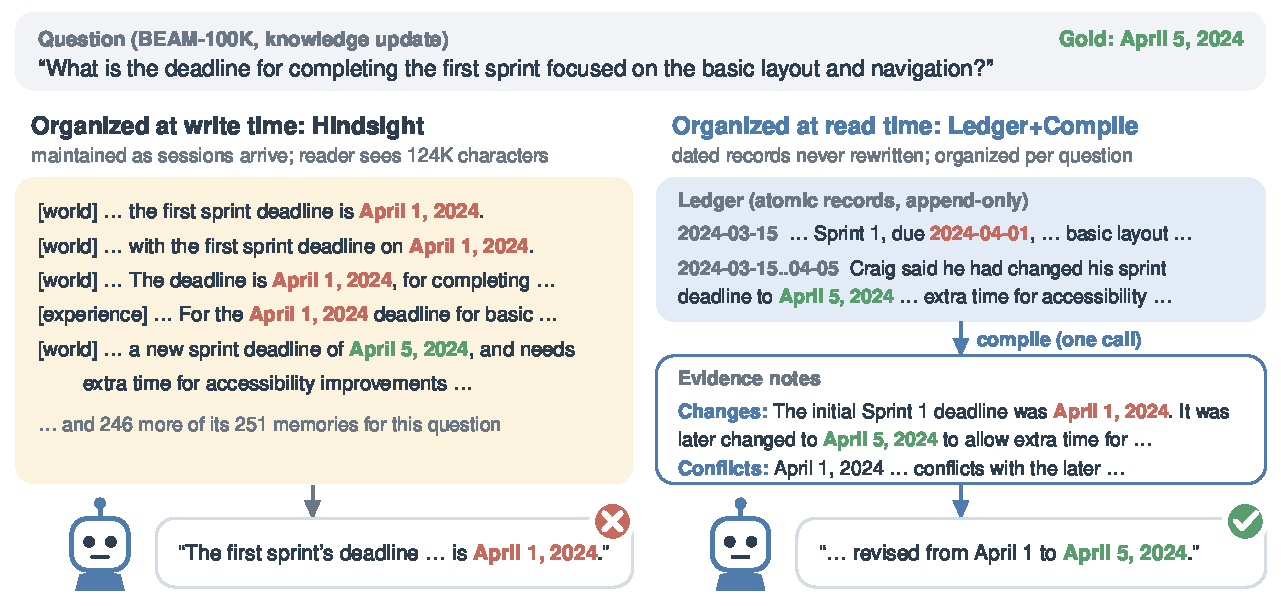
\includegraphics[width=\linewidth]{figs/fig1_teaser.pdf}
\caption{\textbf{The same update, organized at write time and at read time.} A BEAM-100K question whose answer changed
during the conversation. Hindsight's context (left, 251 memories) contains the update, but as one memory among several
that repeat the old date, and the reader gives the old date in all three runs. \method{} keeps both dated records in
its ledger and compiles them for this question into notes that state the change (right); the reader is correct in all
three runs. Quoted text is excerpted from the actual contexts (gpt-6-luna reader, tuned prompt).}
\label{fig:teaser}
\end{figure}

% P3: what we do (A/B round 1: slightly better than ReadAgent's method paragraph; edits applied)
This paper makes that comparison under controlled conditions. We fix a protocol in which only the memory varies:
one reader model, one answer prompt, the official BEAM rubric judge, three independent generations per question, and
confidence intervals clustered by conversation (\cref{sec:setting}). Under this protocol we audit where the scores of
current systems come from, separating the answer prompt, the context budget, and the storage representation
(\cref{sec:audit}). The audit points to the reader as the bottleneck. Of the \prelim{36} points Hindsight loses on
BEAM-1M, \prelim{19.6} come from questions whose answer was already in its context, where the reader did not find
it, did not line up the dates, or did not notice that two statements disagree. Since what a reader needs depends on
the question, we propose to defer organization until the question is known. \method{} (\cref{fig:teaser,fig:overview},
\cref{sec:method}) moves merging, reconciling, and summarizing from write time to read time. The write side only
splits sessions into atomic records and appends them to a ledger that is never rewritten. At question time,
\method{} (1) retrieves a large candidate set of records with hybrid search, (2) compiles them in one call into
question-specific evidence notes (a step we call \emph{compilation}), and (3) gives the reader these notes together with the retrieved records. The
notes order the relevant facts in time and flag updates, conflicts, gaps in coverage, and standing instructions from
the user. We compare against baselines given the same extra call, report the cost of each system, and repeat the main
comparison with three reader models and on LongMemEval~\citep{wu2025longmemeval} (\cref{sec:experiments}).

% P4: findings (A/B round 1: LongMemEval slightly better; round 2 after rewrite: ours slightly better; edits applied)
Our experiments on BEAM at the 100K and 1M tiers and on LongMemEval-S support four findings. Hindsight
always receives an extra read-time call of its own (a conflict check), so no gain below comes from \method{} making
one more call.
\begin{itemize}
\item (\cref{sec:audit}) \textbf{Comparisons at default settings confound storage format with context budget.} On the
100 BEAM-1M development questions, raising Hindsight's budget from 8K to its full 124K characters moves it by
\prelim{25.0} points, while atomic records stay within \prelim{2.1} points at every budget; at equal budgets the format
effect is small and changes sign, from \prelim{$+1.6$} for records at 60K characters to \prelim{$-3.1$} at 124K.
\item (\cref{sec:main,sec:reader}) \textbf{Compiling notes at read time helps, most with a weaker reader.} With
gpt-6-luna as the reader, \method{} leads Hindsight by \prelim{$+7.3$} points on BEAM-100K and \prelim{$+4.2$}
on BEAM-1M (three runs, 95\% intervals above zero). Three stronger readers (DeepSeek-V4.1-Flash, gpt-6.1-sol,
gpt-6-astra) raise Hindsight by \prelim{6} to \prelim{10} points with its memory unchanged, while \method{} gains less;
it stays ahead in all eight reader-and-tier cells, but by only \prelim{1} to \prelim{3} points.
\item (\cref{sec:ablation}) \textbf{Storage format matters once records are compiled into notes.} Notes compiled from
the atomic records that \method{} stores beat the same notes compiled from Hindsight's facts by \prelim{$+6.6$} points on BEAM-100K questions about a single fact or state (95\% interval \prelim{$[+2.6, +11.0]$}), although the
two formats are close when the reader reads them directly (\cref{sec:audit}).
\item (\cref{sec:ablation}) \textbf{Compiled notes are robust to the answer prompt.} The answer prompt that Mem0
published for BEAM adds between \prelim{$+0.7$} and \prelim{$+11.5$} points to systems without notes on BEAM point questions,
but changes the score of compiled notes by at most \prelim{2.3}. On LongMemEval-S the same tuned prompt lowers plain
record retrieval by about \prelim{5} points; with the minimal prompt, \method{} is at or above record retrieval and
Hindsight for all three readers (\cref{tab:lme}).
\end{itemize}

% P5: contributions
In summary, we contribute (i) a controlled protocol and audit that separate the memory from the reader, prompt,
budget, and judge on a 1M-token benchmark; (ii) \method{}, a memory that keeps an append-only ledger and organizes
only at read time, with a compilation format designed for conversational memory; and (iii) evidence across three
readers, two benchmark tiers, and LongMemEval for when read-time organization pays off and when it does not.
\todo{test-set results (BEAM-100K test conversations, BEAM-1M test rows, LongMemEval-S test) once the method is frozen.}
